\section{Cenário de Teste 2}

Este cenário está dividido em 5 (cinco) exemplos, os quais são apresentados a seguir, contemplando todo o processo de auto-localização
em cada exemplo, a partir da apresentação das Imagens abaixo.

\subsection{Exemplo 1}

Exemplo utilizando velocidade de rotação em 10 graus por segundo:

{\centering
\includegraphics[scale=0.4]{figuras/cen2_ex1.eps}
\captionof{figure}{Cenário 2 - Exemplo 1}
\label{img:cen2_ex1}
\par}

\subsection{Exemplo 2}

Exemplo utilizando velocidade de rotação em 30 graus por segundo:

{\centering
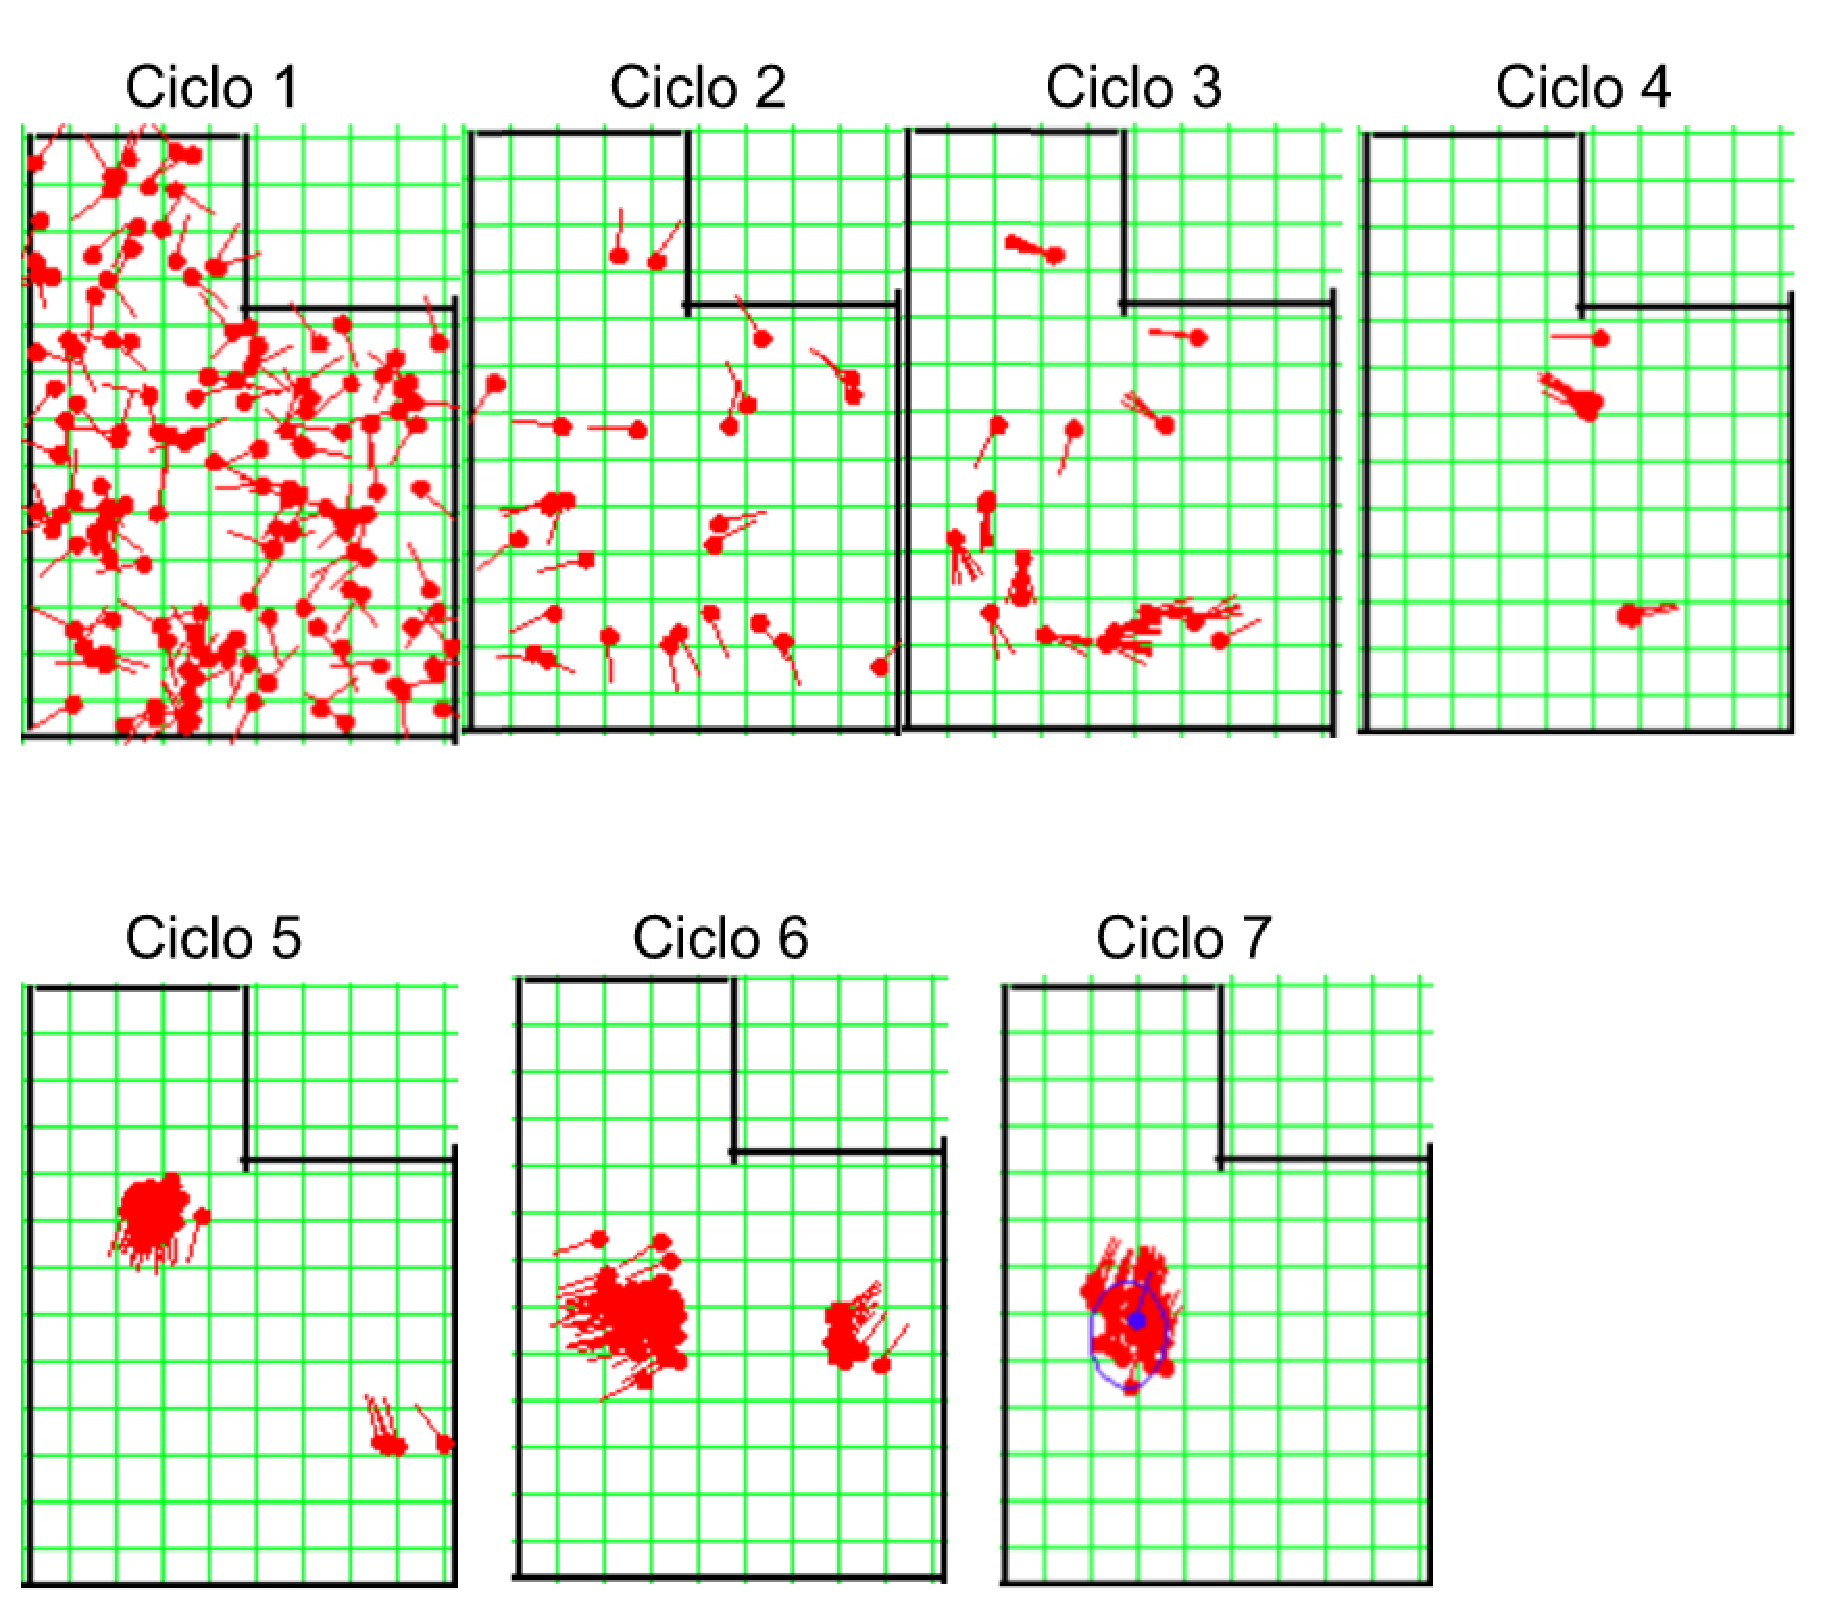
\includegraphics[scale=0.4]{figuras/cen2_ex2.eps}
\captionof{figure}{Cenário 2 - Exemplo 2}
\label{img:cen2_ex2}
\par}

\subsection{Exemplo 3}

Exemplo utilizando velocidade de rotação em 50 graus por segundo:

{\centering
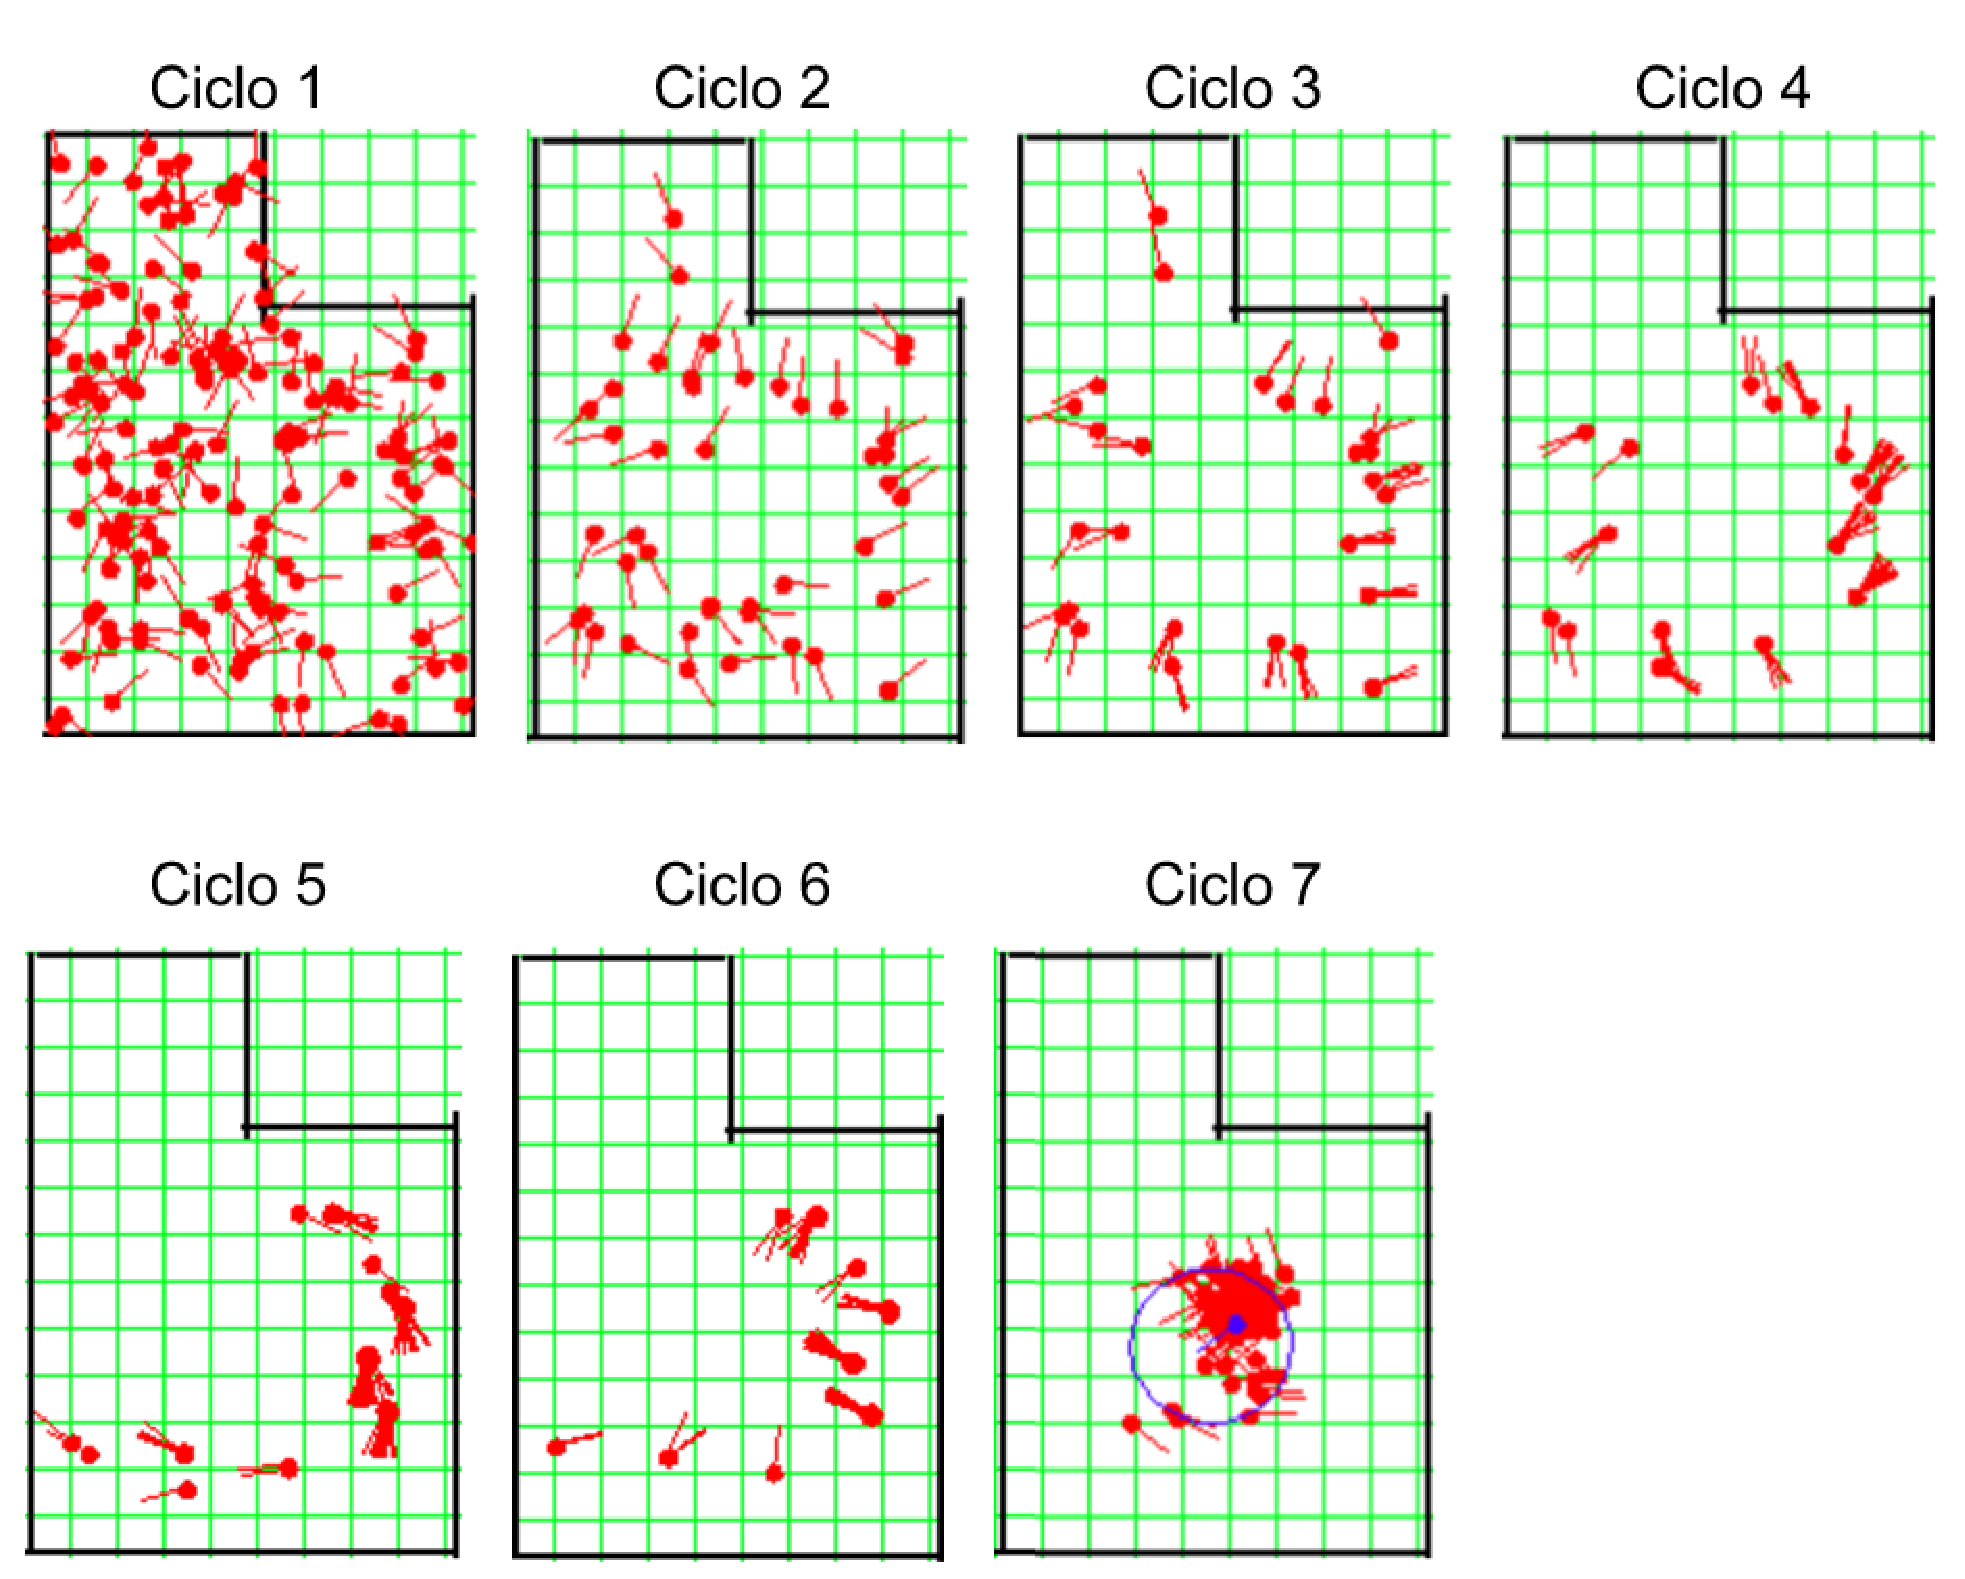
\includegraphics[scale=0.4]{figuras/cen2_ex3.eps}
\captionof{figure}{Cenário 2 - Exemplo 3}
\label{img:cen2_ex3}
\par}

\subsection{Exemplo 4}

Exemplo utilizando velocidade de rotação em 70 graus por segundo:

{\centering
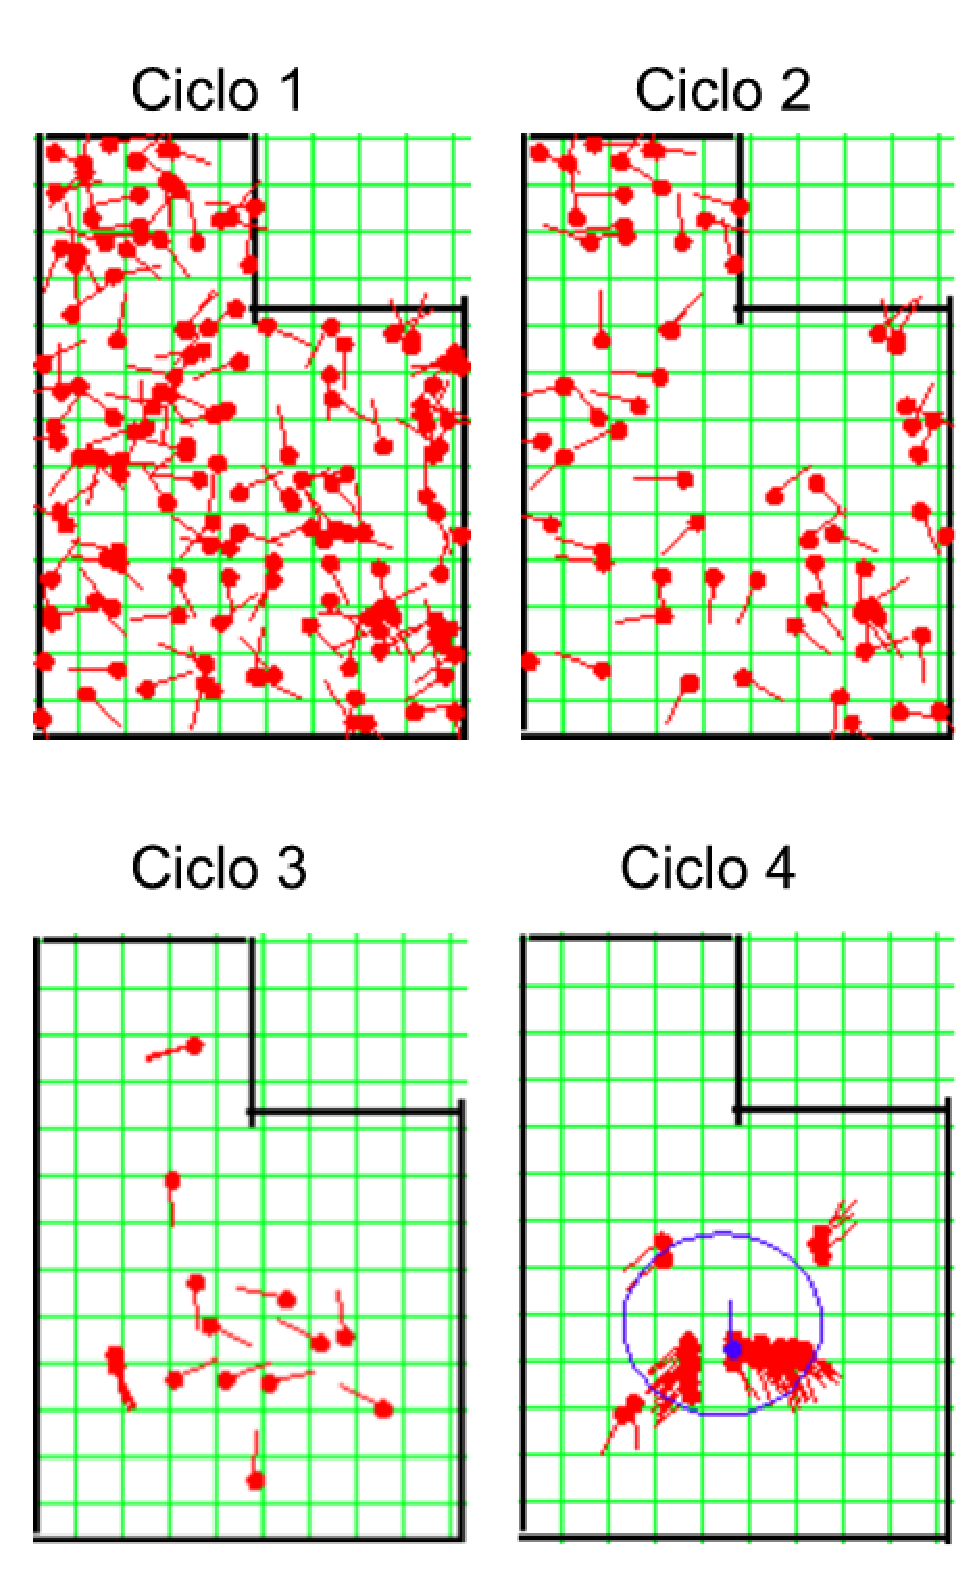
\includegraphics[scale=0.4]{figuras/cen2_ex4.eps}
\captionof{figure}{Cenário 2 - Exemplo 4}
\label{img:cen2_ex4}
\par}

\subsection{Exemplo 5}

Exemplo utilizando velocidade de rotação em 90 graus por segundo:

{\centering
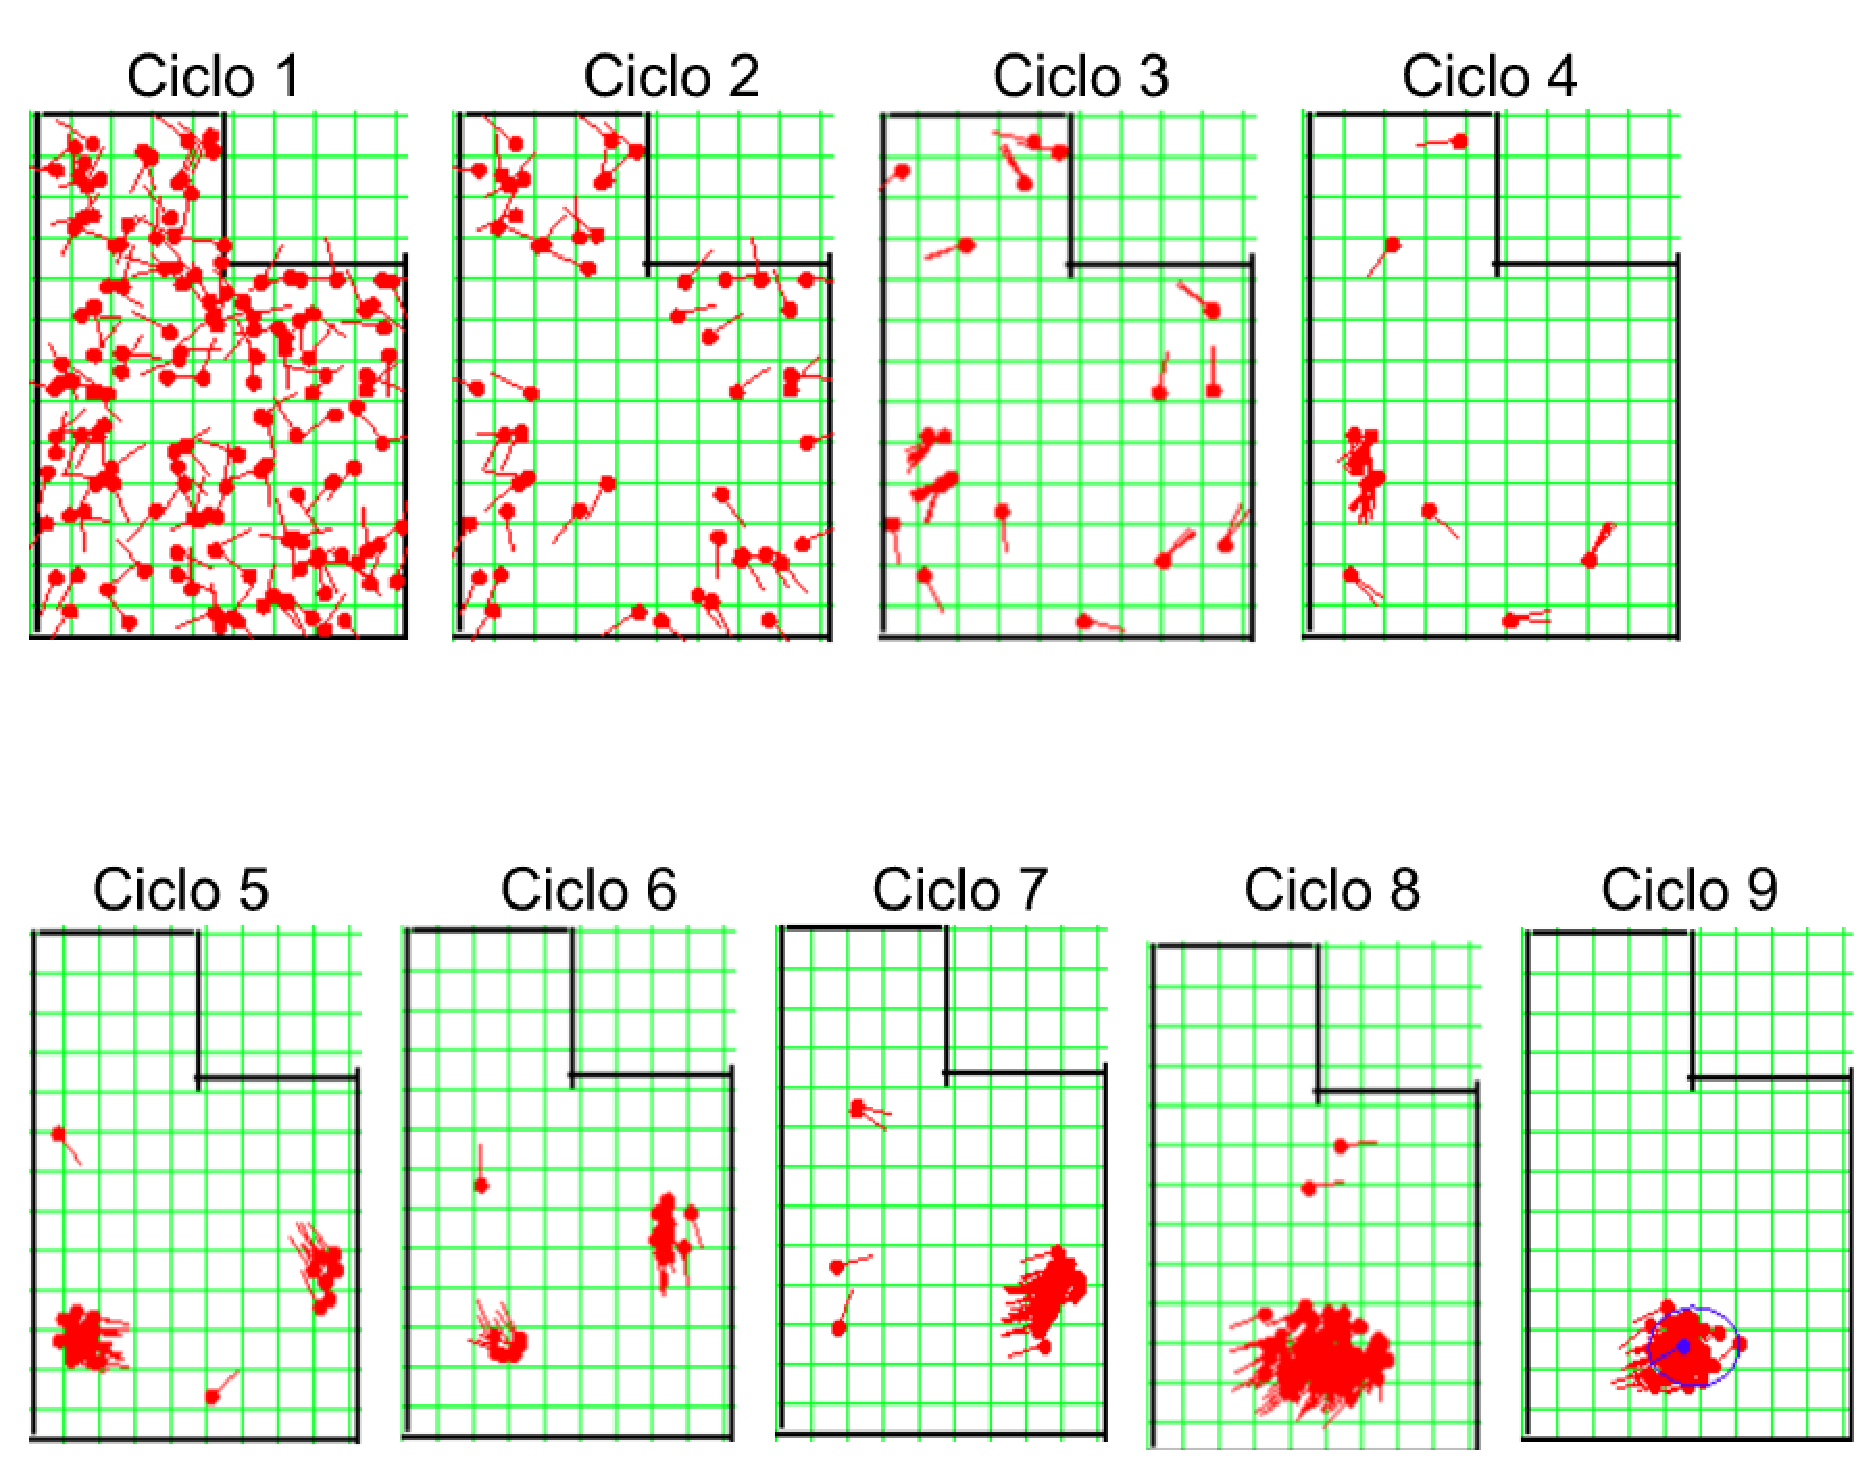
\includegraphics[scale=0.4]{figuras/cen2_ex5.eps}
\captionof{figure}{Cenário 2 - Exemplo 5}
\label{img:cen2_ex5}
\par}
